\documentclass[tikz,border=8pt]{standalone}
% Shared look for every TikZ diagram. Load with % Shared look for every TikZ diagram. Load with % Shared look for every TikZ diagram. Load with \input{../../tools/tikz-style.tex}
\usepackage[T1]{fontenc}
\usepackage{lmodern}
\renewcommand{\sfdefault}{lmr}  % diagrams use the same serif as the text
\usetikzlibrary{arrows.meta, positioning, shapes.geometric, calc, fit, backgrounds}
\definecolor{cblue}{HTML}{4C78A8}
\definecolor{corange}{HTML}{F58518}
\definecolor{cgreen}{HTML}{54A24B}
\definecolor{cred}{HTML}{E45756}
\definecolor{cpurple}{HTML}{B279A2}
\definecolor{cgrey}{HTML}{6B6B6B}
\tikzset{
  every picture/.style={font=\sffamily, line width=1.2pt},
  box/.style={draw=#1, fill=#1!12, rounded corners=4pt, align=center, inner sep=7pt, minimum height=1.1cm},
  box/.default=cgrey,
  arrow/.style={-{Stealth[length=3mm]}, draw=cgrey, line width=1.4pt},
  title/.style={font=\sffamily\bfseries\Large},
  note/.style={font=\sffamily\small, text=cgrey, align=center},
}
\AtBeginDocument{\hyphenpenalty=10000 \exhyphenpenalty=10000}

\usepackage[T1]{fontenc}
\usepackage{lmodern}
\renewcommand{\sfdefault}{lmr}  % diagrams use the same serif as the text
\usetikzlibrary{arrows.meta, positioning, shapes.geometric, calc, fit, backgrounds}
\definecolor{cblue}{HTML}{4C78A8}
\definecolor{corange}{HTML}{F58518}
\definecolor{cgreen}{HTML}{54A24B}
\definecolor{cred}{HTML}{E45756}
\definecolor{cpurple}{HTML}{B279A2}
\definecolor{cgrey}{HTML}{6B6B6B}
\tikzset{
  every picture/.style={font=\sffamily, line width=1.2pt},
  box/.style={draw=#1, fill=#1!12, rounded corners=4pt, align=center, inner sep=7pt, minimum height=1.1cm},
  box/.default=cgrey,
  arrow/.style={-{Stealth[length=3mm]}, draw=cgrey, line width=1.4pt},
  title/.style={font=\sffamily\bfseries\Large},
  note/.style={font=\sffamily\small, text=cgrey, align=center},
}
\AtBeginDocument{\hyphenpenalty=10000 \exhyphenpenalty=10000}

\usepackage[T1]{fontenc}
\usepackage{lmodern}
\renewcommand{\sfdefault}{lmr}  % diagrams use the same serif as the text
\usetikzlibrary{arrows.meta, positioning, shapes.geometric, calc, fit, backgrounds}
\definecolor{cblue}{HTML}{4C78A8}
\definecolor{corange}{HTML}{F58518}
\definecolor{cgreen}{HTML}{54A24B}
\definecolor{cred}{HTML}{E45756}
\definecolor{cpurple}{HTML}{B279A2}
\definecolor{cgrey}{HTML}{6B6B6B}
\tikzset{
  every picture/.style={font=\sffamily, line width=1.2pt},
  box/.style={draw=#1, fill=#1!12, rounded corners=4pt, align=center, inner sep=7pt, minimum height=1.1cm},
  box/.default=cgrey,
  arrow/.style={-{Stealth[length=3mm]}, draw=cgrey, line width=1.4pt},
  title/.style={font=\sffamily\bfseries\Large},
  note/.style={font=\sffamily\small, text=cgrey, align=center},
}
\AtBeginDocument{\hyphenpenalty=10000 \exhyphenpenalty=10000}

\begin{document}
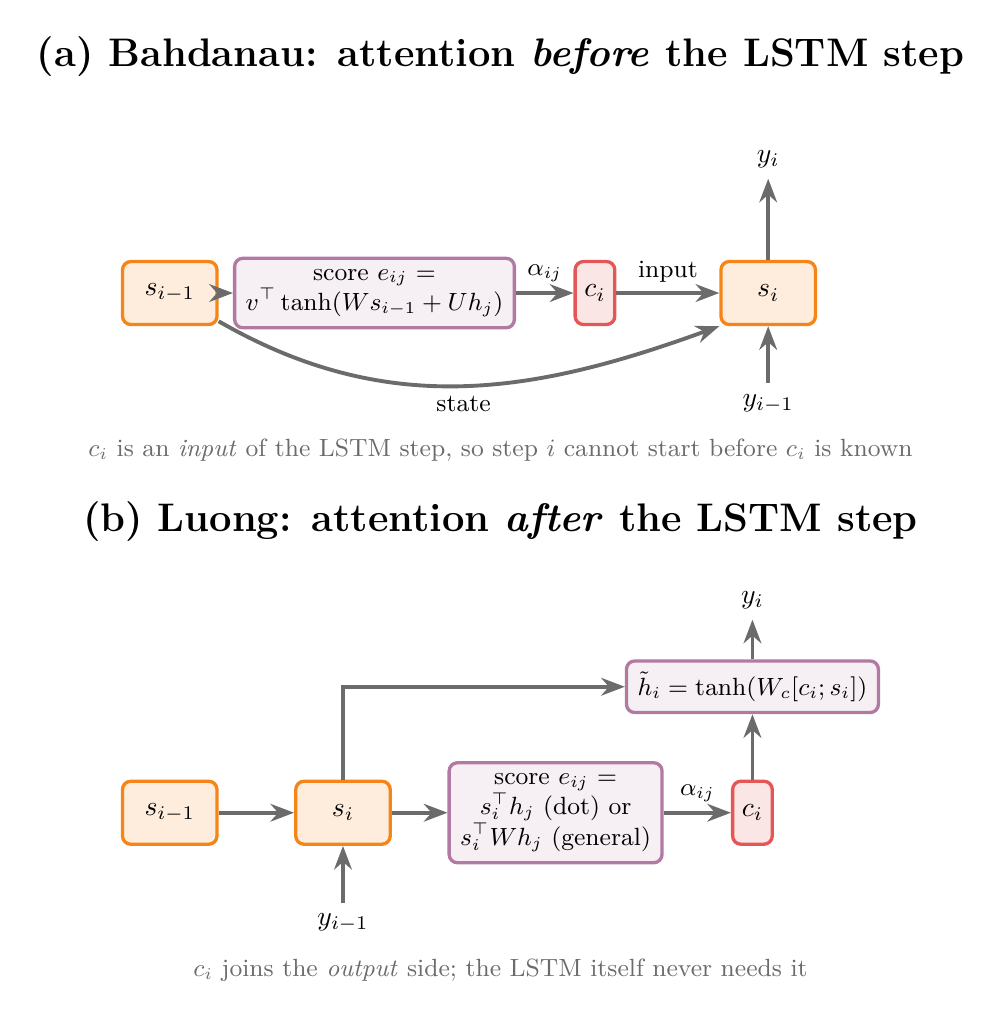
\begin{tikzpicture}[st/.style={draw=corange, fill=corange!15, rounded corners=3pt, minimum width=1.2cm, minimum height=0.8cm, font=\sffamily},
  att/.style={draw=cpurple, fill=cpurple!12, rounded corners=3pt, align=center, font=\sffamily\small, inner sep=4pt},
  cv/.style={draw=cred, fill=cred!15, rounded corners=3pt, font=\sffamily, minimum height=0.8cm},
  word/.style={font=\sffamily}]
  % Bahdanau
  \node[title] at (4.2, 3.0) {(a) Bahdanau: attention \emph{before} the LSTM step};
  \node[st] (sp) at (0, 0) {$s_{i-1}$};
  \node[att] (a1) at (2.6, 0) {score $e_{ij}$ =\\$v^\top\tanh(W s_{i-1} + U h_j)$};
  \node[cv] (c1) at (5.4, 0) {$c_i$};
  \node[st] (si) at (7.6, 0) {$s_i$};
  \node[word] (yp) at (7.6, -1.4) {$y_{i-1}$};
  \node[word] (yo) at (7.6, 1.7) {$y_i$};
  \draw[arrow] (sp) -- (a1); \draw[arrow] (a1) -- node[above, font=\sffamily\small] {$\alpha_{ij}$} (c1); \draw[arrow] (c1) -- node[above, font=\sffamily\small] {input} (si);
  \draw[arrow] (yp) -- (si); \draw[arrow] (si) -- (yo);
  \draw[arrow] (sp) to[out=-30, in=200] node[below, font=\sffamily\small] {state} (si.south west);
  \node[note] at (4.2, -2.0) {$c_i$ is an \emph{input} of the LSTM step, so step $i$ cannot start before $c_i$ is known};
  % Luong
  \begin{scope}[yshift=-6.6cm]
  \node[title] at (4.2, 3.7) {(b) Luong: attention \emph{after} the LSTM step};
  \node[st] (sp2) at (0, 0) {$s_{i-1}$};
  \node[st] (si2) at (2.2, 0) {$s_i$};
  \node[word] (yp2) at (2.2, -1.4) {$y_{i-1}$};
  \node[att] (a2) at (4.9, 0) {score $e_{ij}$ =\\$s_i^\top h_j$ (dot) or\\$s_i^\top W h_j$ (general)};
  \node[cv] (c2) at (7.4, 0) {$c_i$};
  \node[att] (ht) at (7.4, 1.6) {$\tilde{h}_i = \tanh(W_c[c_i; s_i])$};
  \node[word] (yo2) at (7.4, 2.7) {$y_i$};
  \draw[arrow] (sp2) -- (si2); \draw[arrow] (yp2) -- (si2); \draw[arrow] (si2) -- (a2);
  \draw[arrow] (a2) -- node[above, font=\sffamily\small] {$\alpha_{ij}$} (c2); \draw[arrow] (c2) -- (ht); \draw[arrow] (ht) -- (yo2);
  \draw[arrow] (si2) |- (ht);
  \node[note] at (4.2, -2.0) {$c_i$ joins the \emph{output} side; the LSTM itself never needs it};
  \end{scope}
\end{tikzpicture}
\end{document}
